% Séquence 4 : Distance, cercle et triangles
\setseqtitle{Distance, cercle et triangles}
\chapter{Distance, cercle et triangles}

\begin{objectifsbox}
	\textbf{Objectifs d'apprentissage de la séquence}
	\begin{itemize}
		\item Connaître et utiliser la définition de la distance entre deux points
		\item Connaître et utiliser la définition du milieu d'un segment
		\item Connaître les définitions d'un cercle, d'un disque, d'un rayon, d'un diamètre, d'une corde
		\item Comprendre la définition d'un cercle et celle d'un disque sous la forme d'ensembles de points
		\item Construire des triangles
		\item Résoudre des problèmes mettant en jeu des distances à un point
	\end{itemize}
\end{objectifsbox}

\section{Distance entre deux points}

\begin{definitionbox}
	\textbf{Distance entre deux points}
	
	La distance entre deux points A et B est \trous{5cm}.
	
	On la note \trous{3cm} et on peut également noter \trous{3cm}.
\end{definitionbox}

\textbf{Propriétés importantes :}
\begin{itemize}
	\item La distance entre deux points est toujours \trous{3cm}
	\item La distance d'un point A à un point B est \trous{5cm} que la distance du point B au point A
	\item On peut noter : \trous{4cm}
\end{itemize}

\textbf{Remarque :} Ne pas oublier l'unité de longueur !

\begin{examplebox}
	Soient 3 points O, P et M tels que OM = 3 cm, MP = 5 cm et OP = 8 cm.
	Montrer que le point M appartient au segment [OP].
	
	\trous{12cm}
	
	\trous{12cm}
	
	\trous{12cm}
\end{examplebox}

\section{Appartenance à un segment}

\begin{definitionbox}
	\textbf{Points et segments}
	
	Le segment [AB] est \trous{6cm}.
	
	Si le point C n'appartient pas au segment [AB], alors \trous{4cm}.
	
	Si le point D appartient au segment [AB], alors \trous{4cm}.
	
	Pour tout point M, \trous{4cm}.
\end{definitionbox}

Le symbole << $\geqslant$ >> se lit \trous{4cm}.

\textbf{Propriété :} Si AD + DB = AB, alors \trous{6cm}.

\section{Milieu d'un segment}

\begin{definitionbox}
	\textbf{Milieu d'un segment}
	
	Le milieu d'un segment est \trous{8cm}.
	
	<< Équidistant >> signifie << \trous{4cm} >>.
\end{definitionbox}

\begin{examplebox}
	% Schéma avec segment et milieu
	\begin{center}
		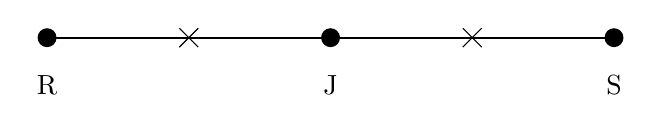
\begin{tikzpicture}[scale=1.2]
			% Segment RS avec milieu J
			\draw[thick] (0,0) -- (6,0);
			\fill (0,0) circle (0.1);
			\fill (6,0) circle (0.1);
			\fill (3,0) circle (0.1);
			
			\node[below] at (0,-0.3) {R};
			\node[below] at (6,-0.3) {S};
			\node[below] at (3,-0.3) {J};
			
			% Codage des segments égaux
			\draw (1.4,-0.1) -- (1.6,0.1);
			\draw (1.4,0.1) -- (1.6,-0.1);
			\draw (4.4,-0.1) -- (4.6,0.1);
			\draw (4.4,0.1) -- (4.6,-0.1);
		\end{tikzpicture}
	\end{center}
	
	J $\in$ [RS] et RJ = JS
	
	Donc \trous{6cm}
	
	Ne pas oublier le codage !
\end{examplebox}

\section{Le cercle}

\begin{definitionbox}
	\textbf{Définitions importantes}
	
	Le cercle de centre O et de rayon r est \trous{8cm}.
	
	Le disque de centre O et de rayon r est \trous{8cm}.
\end{definitionbox}

% Schéma d'un cercle avec vocabulaire
\begin{center}
	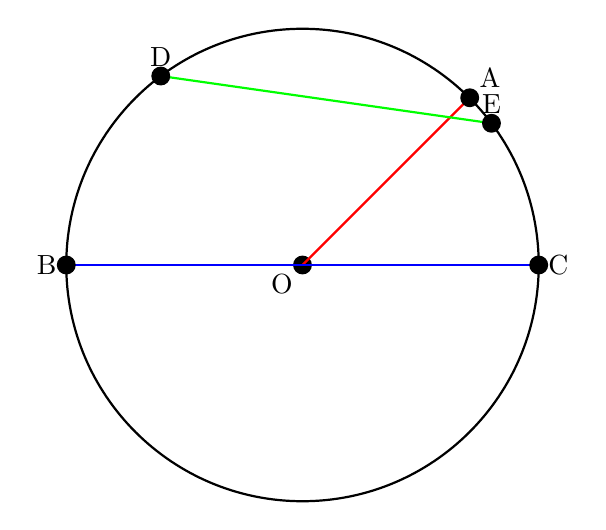
\begin{tikzpicture}[scale=1.2]
		% Cercle
		\draw[thick] (0,0) circle (2.5);
		
		% Centre
		\fill (0,0) circle (0.1);
		\node[below left] at (0,0) {O};
		
		% Rayon
		\draw[thick, red] (0,0) -- (1.77,1.77);
		\fill (1.77,1.77) circle (0.1);
		\node[above right] at (1.77,1.77) {A};
		
		% Diamètre
		\draw[thick, blue] (-2.5,0) -- (2.5,0);
		\fill (-2.5,0) circle (0.1);
		\fill (2.5,0) circle (0.1);
		\node[left] at (-2.5,0) {B};
		\node[right] at (2.5,0) {C};
		
		% Corde
		\draw[thick, green] (-1.5,2) -- (2,1.5);
		\fill (-1.5,2) circle (0.1);
		\fill (2,1.5) circle (0.1);
		\node[above] at (-1.5,2) {D};
		\node[above] at (2,1.5) {E};
	\end{tikzpicture}
\end{center}

\textbf{Vocabulaire :}
\begin{itemize}
	\item OA = \trous{3cm}
	\item [OA] est \trous{3cm}
	\item [BC] est \trous{3cm}
	\item [DE] est \trous{3cm}
	\item DE est \trous{3cm}
\end{itemize}

\section{Utilisation de la définition du cercle}

\begin{examplebox}
	\textbf{Exercice 1 :} Trace l'ensemble de tous les points situés à 5 cm du point O.
	
	\trous{10cm}
	
	\vspace{3cm}
	
	\textbf{Exercice 2 :} Trace et colorie l'ensemble de tous les points situés à plus de 2 cm et à moins de 4 cm du point P.
	
	\trous{10cm}
	
	\vspace{3cm}
\end{examplebox}

\section{Construction d'un triangle équilatéral}

\begin{definitionbox}
	\textbf{Triangle équilatéral}
	
	Un triangle équilatéral est un triangle qui a ses trois côtés de même mesure.
\end{definitionbox}

\textbf{Méthode de construction :}

Pour tracer un triangle équilatéral, on commence par tracer un côté puis, au compas, on trouve son troisième sommet.

\textbf{Points importants :}
\begin{itemize}
	\item On n'oublie pas de placer les noms des sommets
	\item On n'oublie pas le codage pour indiquer que les trois côtés ont la même mesure
	\item Les marques de construction doivent rester visibles
\end{itemize}

\begin{examplebox}
	\textbf{Exemple :} Finis la construction du triangle équilatéral LMN de côté 5 cm.
	
	% Schéma à compléter
	\begin{center}
		\begin{tikzpicture}[scale=1.2]
			% Segment LN déjà tracé
			\draw[thick] (0,0) -- (4,0);
			\fill (0,0) circle (0.1);
			\fill (4,0) circle (0.1);
			\node[below] at (0,-0.3) {L};
			\node[below] at (4,-0.3) {N};
			
			% Arcs de construction (en pointillés)
			\draw[dashed, red] (0,0) circle (4);
			\draw[dashed, blue] (4,0) circle (4);
		\end{tikzpicture}
	\end{center}
	
	\vspace{3cm}
\end{examplebox}

\section{Construction d'un triangle isocèle}

\begin{definitionbox}
	\textbf{Triangle isocèle}
	
	Un triangle isocèle est un triangle qui possède deux côtés de même mesure.
	
	Dire que le triangle ABC est isocèle en A revient à dire que A est son \trous{4cm} et donc que [BC] est sa \trous{3cm}.
	
	[AB] et [AC] sont donc de même mesure.
\end{definitionbox}

\textbf{Méthode de construction :}

Pour tracer un triangle isocèle, on commence par tracer sa base puis, au compas, on trouve son sommet principal.

\begin{examplebox}
	\textbf{Exemple :} Finis la construction du triangle ABC isocèle en A sachant que BC = 3 cm et AB = 5 cm.
	
	% Schéma à compléter
	\begin{center}
		\begin{tikzpicture}[scale=1.2]
			% Base BC déjà tracée
			\draw[thick] (0,0) -- (3,0);
			\fill (0,0) circle (0.1);
			\fill (3,0) circle (0.1);
			\node[below] at (0,-0.3) {B};
			\node[below] at (3,-0.3) {C};
			
			% Arc de construction depuis B
			\draw[dashed, red] (0,0) circle (5);
		\end{tikzpicture}
	\end{center}
	
	\vspace{3cm}
\end{examplebox}

\section{Construction d'un triangle quelconque}

\begin{definitionbox}
	\textbf{Triangle quelconque}
	
	Un triangle quelconque a ses 3 côtés de mesures différentes.
\end{definitionbox}

\textbf{Méthode de construction :}

Pour tracer un triangle quelconque, on commence par tracer son plus long côté. Le troisième sommet se trace avec un compas.

\begin{examplebox}
	\textbf{Exemple 1 :} Finis la construction du triangle ABC sachant que AC = 8 cm, AB = 6 cm et BC = 4 cm.
	
	% Schéma à compléter
	\begin{center}
		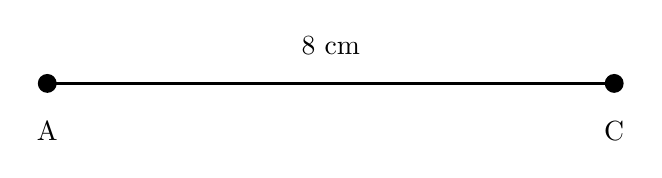
\begin{tikzpicture}[scale=1.2]
			% Le plus long côté AC déjà tracé
			\draw[thick] (0,0) -- (6,0);
			\fill (0,0) circle (0.1);
			\fill (6,0) circle (0.1);
			\node[below] at (0,-0.3) {A};
			\node[below] at (6,-0.3) {C};
			\node[above] at (3,0.2) {8 cm};
		\end{tikzpicture}
	\end{center}
	
	\vspace{3cm}
	
	\textbf{Exemple 2 :} Trace un triangle EFG sachant que EF = 10 cm, FG = 8 cm et EG = 5 cm.
	
	\vspace{4cm}
\end{examplebox}

\textbf{Remarques importantes :}
\begin{itemize}
	\item Les marques de construction doivent rester visibles
	\item Ne pas oublier de nommer les 3 sommets
\end{itemize}

\section{Construction d'un triangle rectangle}

\begin{definitionbox}
	\textbf{Triangle rectangle}
	
	Un triangle rectangle est un triangle qui possède un angle droit.
\end{definitionbox}

\textbf{Méthode de construction :}

Pour tracer un triangle rectangle, on commence par tracer les 2 côtés de l'angle droit avec une règle et une équerre puis on reporte les longueurs connues.

\textbf{Points importants :}
\begin{itemize}
	\item On n'oublie pas de placer les noms des sommets
	\item On n'oublie pas le codage pour indiquer l'angle droit
\end{itemize}

\begin{examplebox}
	\textbf{Exemple 1 :} Finis la construction du triangle ABC rectangle en C sachant que AC = 5 cm et BC = 4 cm.
	
	% Schéma à compléter
	\begin{center}
		\begin{tikzpicture}[scale=1.2]
			% Angle droit en C
			\draw[thick] (0,0) -- (4,0);
			\draw[thick] (0,0) -- (0,3);
			\fill (0,0) circle (0.1);
			\node[below left] at (0,0) {C};
			
			% Codage angle droit
			\draw (0.3,0) -- (0.3,0.3) -- (0,0.3);
		\end{tikzpicture}
	\end{center}
	
	\vspace{3cm}
	
	\textbf{Exemple 2 : les 2 côtés de l'angle droit sont connus}
	
	Trace un triangle EFG rectangle en F sachant que EF = 6 cm et FG = 2 cm.
	
	\vspace{3cm}
	
	\textbf{Exemple 3 : un seul côté de l'angle droit est connu}
	
	Trace un triangle MNO rectangle en O sachant que ON = 3 cm et MN = 5 cm.
	
	\vspace{3cm}
\end{examplebox}

\textbf{Exercices d'application :}

\begin{exercisebox}
	1. Construire un triangle équilatéral XYZ de côté 3,5 cm.
	
	\vspace{4cm}
	
	2. Construire un triangle IJK isocèle en J avec IJ = 7 cm et IK = 4 cm.
	
	\vspace{4cm}
	
	3. Les points A, B et C sont-ils alignés si AB = 5 cm, BC = 3 cm et AC = 8 cm ? Justifier.
	
	\trous{8cm}
	
	\trous{8cm}
	
	4. Soit M le milieu du segment [EF]. Si EM = 3,5 cm, quelle est la longueur EF ?
	
	\trous{8cm}
\end{exercisebox}